\documentclass[12pt]{article}
\usepackage{mathtools, amsmath, amsfonts, amssymb, siunitx,array}
\usepackage{hyperref, graphicx, wrapfig, geometry}
\usepackage[makeroom]{cancel}
\usepackage{placeins}
\usepackage{float}


\newgeometry{margin=2cm}

\title{Microprocessor Systems - Final Report}
\author{Auguste Lalande, Felix Dube, Juan Morency Trudel}
\date{\today}

\begin{document}
\maketitle
\clearpage

\tableofcontents
\clearpage

\section{Abstract}
An android application was designed to interact with an embedded system using Bluetooth Low Energy (BLE). The goal of this system was the monitoring of sensor readings and transmission of control signals to the embedded side. The resulting low resource system is responsive and equipped with a polished UI. Phone applications that interact with embedded systems are proved accessible and useful for consumer electronics.
\section{Problem Statement}
This project consisted of establishing full duplex communication between a cellphone and an embedded system through Bluetooth. For this purpose, a STM32F407 microcontroller mounted on a STMF4Discovery board was to be used on the embedded side to gather information from sensors and control LEDS. Furthermore, the STM32F4xx Cube HAL drivers can facilitate software development. On the cellphone side, an Android device was to be used for the user interface (UI). Since the STMF4Discovery board is not equipped with any Bluetooth functionality, an intermediate STM32F401RE Nucleo Board with a DB04A1 BLE Shield was required. The functionalities to be implemented on this triple unit system are listed below:

\begin{enumerate}
\item Temperature monitoring of the STM32F407 microcontroller on the android device.
\item Transmission of filtered 3D accelerometer values from the Discovery board to the android device.
\item Double tap on the discovery board to wake up the phone.
\item Control over four LEDs on the Discovery board from the phone.
\item Efficient wired communication protocol between the discovery board and the nucleo board as well as a wireless protocol between the nucleo board and the android phone.
\item A user interface on an android application must be developed for efficient visualization of the sensor readings as well as flexible control over the LEDs.
\end{enumerate}
\section{Theory and Hypothesis}
\subsection{Pulse Width Modulation}
Pulse Width Modulation (PWM) is a modulation technique that allows the control of the power transferred to a load. As the name states, it consist in using a high-frequency clock (much higher than what would affect the load) to control the length of pulses and the time period between them. PWM can be used to control brightness of a LED by letting current flow only a certain percentage of a time period \cite{PWMLED}. This percentage is called the duty cycle and is easily visualize in figure \ref{fig:pwm}. If the complete cycle frequency is much faster than the human eye can perceive, then no flickering is apparent and the LED simply appears dimmer. Thus, PWM allows the precise control over the brightness of a LED.

\begin{figure}[!htb]
  \centering
  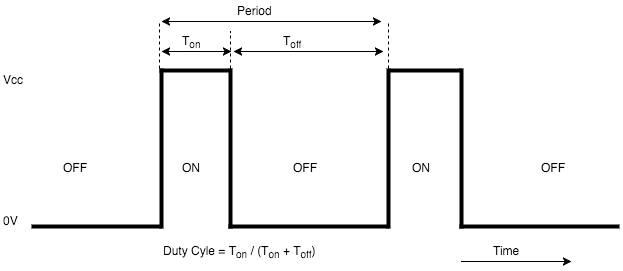
\includegraphics[scale=0.65]{images/PWM.png}
  \caption{Pulse Width Modulation Graphical Explanation}
  \label{fig:pwm}
 \end{figure}

\subsection{Double Tap Feature}
Double tap (DT) was recently introduced on the android platform to easily wake up cellphones without pressing any hardware button by simply double tapping on the screen. The only sensor required for this feature is a 3D accelerometer, which most smartphones already come equipped with. Taps can easily be detected as spikes in the raw value of the acceleration input. By filtering out low-frequency noise from phone movements, a tap can be detected without any false positives. Controlling the delay between taps and other timing parameters can also help improve the filtering of taps. With the right filtering algorithm even light double taps can be detected from any initial position and this with minimum resources.

\subsection{SPI Communication}
The serial peripheral interface (SPI) protocol is a four wire, full duplex, serial interface specification ideal for short range communication between embedded devices. As seen in figure \ref{fig:spi}, the implementation uses two data lines, one clock line, and one slave select line \cite{SPIprotocol}. The data lines are divided into the master in slave out (MISO) on which data travels from slave to master and the master out slave in (MOSI) on which data travels from master to slave. All communication is synced to the master's clock which is set on the clock line (SCLK). Finally, the slave select line (SSL) is used by the master to indicate which slave it is communicating with. In the case where there is only one slave the line can be kept permanently high.

\begin{figure}[!htb]
  \centering
  \includegraphics[scale=0.65]{images/spi.png}
  \caption{SPI Communication Overview}
  \label{fig:spi}
 \end{figure}

\subsection{Bluetooth Low Energy}
Bluetooth Low Energy (BLE) allows wireless communication between different compliant devices. The Generic Attribute Profile (GATT) is the protocol used to exchange data over BLE connection \cite{BLEGATT}. First of all, GATT requires the definition of the different roles of the connected devices. A device can either be a server or a client. If the device is a server, it will receive and send responses to the clients. It will also store and make data available to the clients. If the device is a client it will send requests to a server and receive responses from it.
\paragraph{}
Moreover, GATT uses the Attribute Protocol (ATT) as its transport protocol. The ATT defines how the data is organized. In the GATT server, data is separated in different sections called services. Each service holds one to many characteristics, and these characteristics are what contains the user data. Figure \ref{fig:gatt} illustrates the data structure introduced by GATT.

\begin{figure}[!htb]
 \centering
 \includegraphics[scale=0.65]{images/GATT.png}
 \caption{GATT Server Overview}
 \label{fig:gatt}
\end{figure}

Each characteristic can have different properties:
\begin{itemize}
\item Read property: the client can read the data that it contains.
\item Write property: the client can modify the data that the characteristic holds.
\item Notify property: the server can send notifications to different characteristics.
\end{itemize}

\subsection{Android}
An Android phone is a good device for designing user interface because of its flexibility and availability. Connection with other devices can be realized using many different wireless communication protocol, including BLE. Additionally, Android application can be easily built using a highly documented development environment called Android Studio.

\section{Implementation}
The implementation of the software on the discovery board is done by recycling the concepts employed in previous experiments \cite{Lab2report}\cite{Lab4report}. A multi-threaded operating system is used to simplify the software. The reader can refer to these previous reports for more information. The new features implemented in this project are described in the following sections.

\subsection{LED Control}
Four LEDs are used on the nucleo board for visual feedback. These are hard-wired to PWM compliant ports on the microcontroller. Three LED modes are implemented and can be selected from the android application:
\begin{enumerate}
\item All four LEDs ON mode
\item All four LEDs OFF mode
\item Rotating LED mode where the LEDs take turn being lit in a rotating manner. The speed and direction of the rotation can also be controlled from the Android side.
\end{enumerate}
Independent to the mode selected, the brightness of each LED can be tuned by the use of PWM. A hardware timer at 10 MHz frequency is used to adjust the PWM duty cycle. As a result, precise individual LED brightness is achieved.

\subsection{Double Tap feature}
The double tap (DT) feature is successfully implemented to notify the android device. Important filtering was necessary to avoid triggering DT by simply moving the discovery board. The FSM diagram presented in figure \ref{fig:FSMDT} in the appendix gives an overview of the different methods used to avoid false positives. To understand why filtering is implemented this way, please refer to the testing section. The accelerometer used for this feature was calibrated using the method from \cite{Lab4report}. The raw values of the accelerometer are used for this algorithm to detect spikes as opposed to the filtered values from the kalman filter described in \cite{Lab2report} which would filter out fast variations. Next is a brief description of the mechanisms elaborated with the goal of detecting double taps efficiently.
\paragraph{}
First the algorithm waits for the acceleration value to have an increase followed by a decrease or vice versa and records this as a spike. The amplitude of the increase or decrease is set to 10 mg for detection of even the smallest taps. Then a small delay of 20 ms is introduced as a relaxation time for the accelerometer to settle down in order to avoid reading multiple spikes from a single tap. In the following time period of 40 ms, if a spike is detected, the first tap is neglected. This acts as an apparatus to avoid DT detection from vibration which happens when sliding the board on the table. If 40 ms pass without any other variation, the spike is recorded as a clean spike. The algorithm then waits for a second tap the same way it did for the first one. If a second clean tap is not detected before 250 ms, then the algorithm starts over by waiting for a first tap.
\paragraph{}
The resulting DT detection is very accurate and can consistently detect small double taps even on the table on which the discovery board is placed. False positives from sliding the board on the table or from moving the board in the air were rare, happening fewer than 1\% of the time.
Double tap is implemented independently for x, y and z detection using this technique, which allows the software to determine in what direction the DT was recorded. For 3D DT, a final filtering mechanism is implemented in which if the second tap was not in the same direction as the first one, both taps are neglected. Refer to the code or the FSM (figure \ref{fig:FSMDT}) for more detailed information on our algorithm.

\subsection{SPI Communication}
SPI communication is used to transfer data between the discovery board and the Nucleo board. It is important for the two boards to be able to communicate because only the Nucleo board was equipped with Bluetooth capabilities while the discovery board was used to acquire data.
\paragraph{}
Although HAL drivers were available which already implemented SPI communication, these were found to be difficult to use. Therefore the communication is implemented without the use of said drivers. Instead the Nucleo board waits for a START\_BYTE to be sent by the Discovery board indicating the beginning of communication. After the byte is received the Discovery board starts by transferring the temperature ,accelerometer, and double tap data to the Nucleo board. Once this data is transfered the Nucleo board sends the LED control data to the Discovery board. In the case where the data to be communicated is a float, the discovery board will first convert the IEEE 754 number into a byte array which can then be transferred and converted back to a float by the Nucleo board.
\paragraph{}
In terms of timing, the SPI communication on the discovery board was set to attempt a data transfer every $100 ms$ to ensure that the Nucleo board would eventually detect the data transfer. On the other hand since threads were not available on the Nucleo board, it would simply listen and wait for a START\_BYTE each time it had cycled through its other tasks.

\subsection{Bluetooth Low Energy}
For this project, the GATT server is managed by the Nucleo board using the X-NUCLEO-IDB04A1 Bluetooth shield and only one client--the Android phone--is interacting with the server. An overview of the GATT server is presented in figure \ref{fig:gattimp}.
\paragraph{}

\begin{figure}[!htb]
 \centering
 \includegraphics[scale=0.65]{images/GATTimplementation.png}
 \caption{GATT Server Implementation}
 \label{fig:gattimp}
\end{figure}

The accelerometer service allows the phone to read the roll and pitch values of the discovery board. Similarly, the phone receives information about the temperature of the STM32F407 CPU in the temperature service. The GATT server also holds an LED service, which contains characteristics for which the value would be updated by the phone. Lastly, the Nucleo board can notify the phone using the double tap service, which contains only one characteristic.

\subsection{Android}
The user interface was implemented using Android Studio, and tested on a Samsung Galaxy S6 phone. Using the phone, the user can control different behaviours of the discovery board, and receive data from it. An overview of the application can be seen in figure \ref{fig:android}.
\paragraph{}

\begin{figure}[!htb]
 \centering
 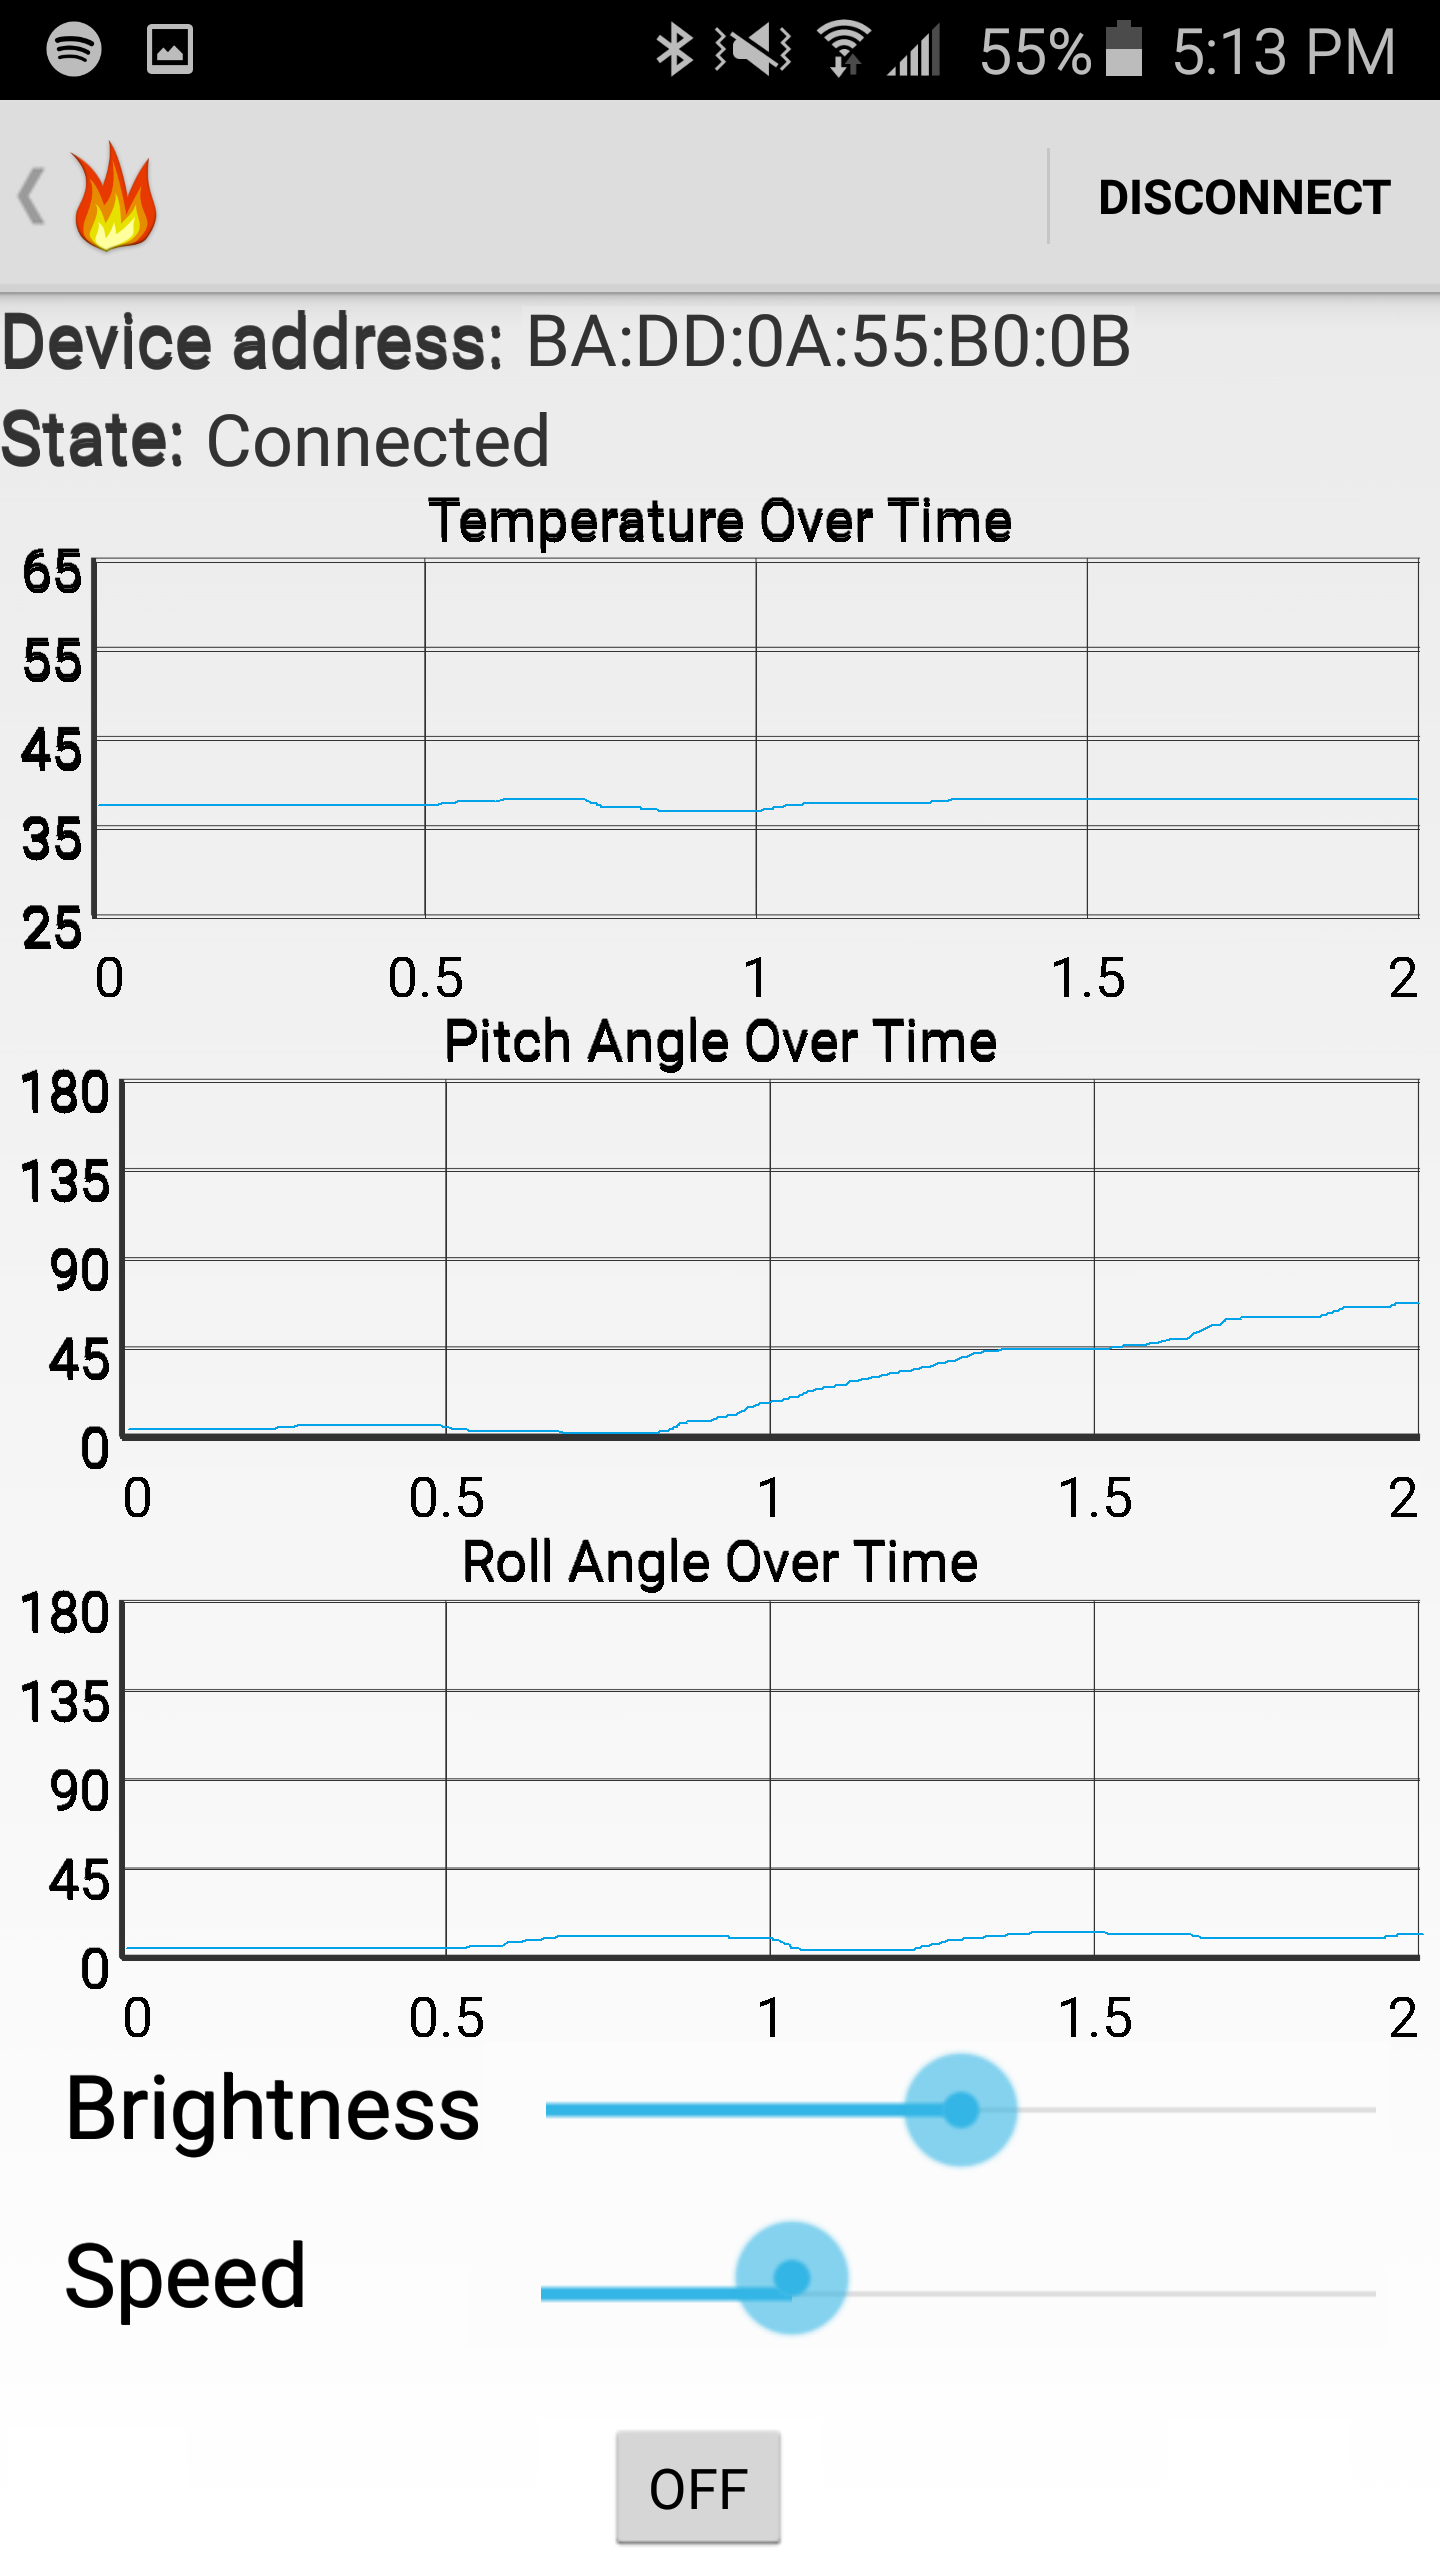
\includegraphics[scale=0.15]{images/android.png}
 \caption{Android Application Main View}
 \label{fig:android}
\end{figure}

First of all, the temperature, roll, and pitch data are presented to the user using a graph from the Graph View library. For each of the values, a thread has been set up to read the Bluetooth characteristic and update the data points that are displayed on the graph every 20 milliseconds. The main thread would then update the graphs with the new data points.
\paragraph{}
Secondly, the UI contains two sliders, which control the speed and brightness of the LEDs on the Discovery board. A listener has been instantiated for each of the sliders. When the user moves a slider the listener calls a function that writes the new value to the specific characteristic. The UI also contains a button which allows the user to turn the LEDs on or off.
\paragraph{}
Lastly, when the double tap characteristic gets notified an Android notification is displayed on the screen. If the phone is sleeping, the screen wakes up to display the notification.


\section{Testing and Observations}
When the system was fully functional, formal testing was kept to a minimal because this system is simply designed to demonstrate the communication functionalities with an embedded system and is not meant for commercialization. For example, testing of the communication between the board and over the Bluetooth connection was judged unnecessary because of the robustness of our SPI and BLE protocols. Also, from the multiple times the system was tried, the communication never appeared to fail regardless of the order of booting of the 3 devices. Testing of the android application was done on a Samsung Galaxy S6 phone as mentioned previously. The only feature of our system that required extensive testing was Double Tap, which is explained in the next section.
\subsection{Double Tap}
First graphs of the raw acceleration value of when a double tap and other undesirable event happened were analyzed (figures \ref{fig:DTCAL1}, \ref{fig:DTCAL2}, \ref{fig:DTCAL3}). From these results, the filtering algorithm described above was implemented. The following observations guided the design of the algorithm:

\begin{figure}[!htb]
 \centering
 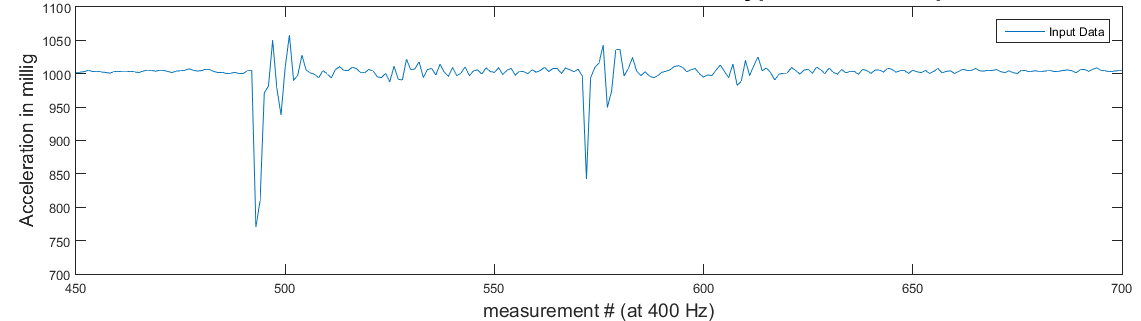
\includegraphics[scale=0.45]{images/DTcalibration1.png}
 \caption{Raw Acceleration Measurements from 3 Successive Double Taps}
 \label{fig:DTCAL1}
\end{figure}

\begin{figure}[!htb]
 \centering
 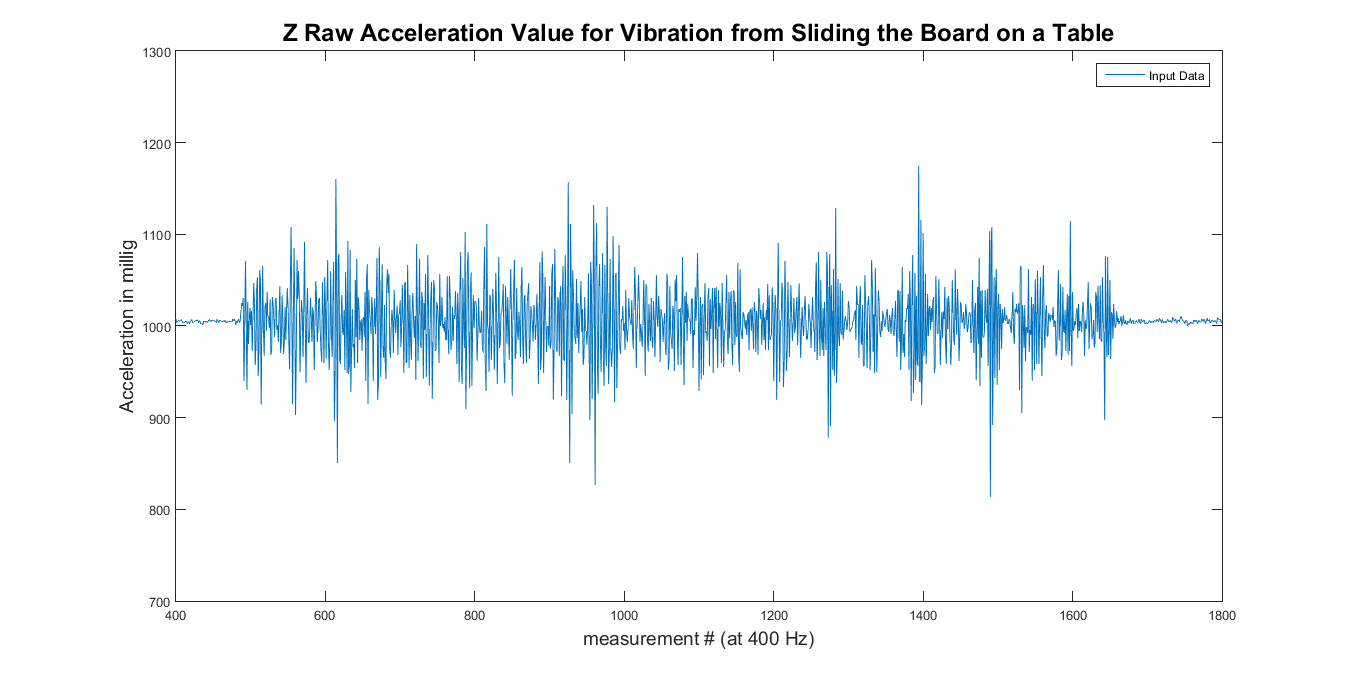
\includegraphics[scale=0.45]{images/DTcalibration2.png}
 \caption{Raw Acceleration Measurements from Sliding the Board on the Table}
 \label{fig:DTCAL2}
\end{figure}

\begin{figure}[!htb]
 \centering
 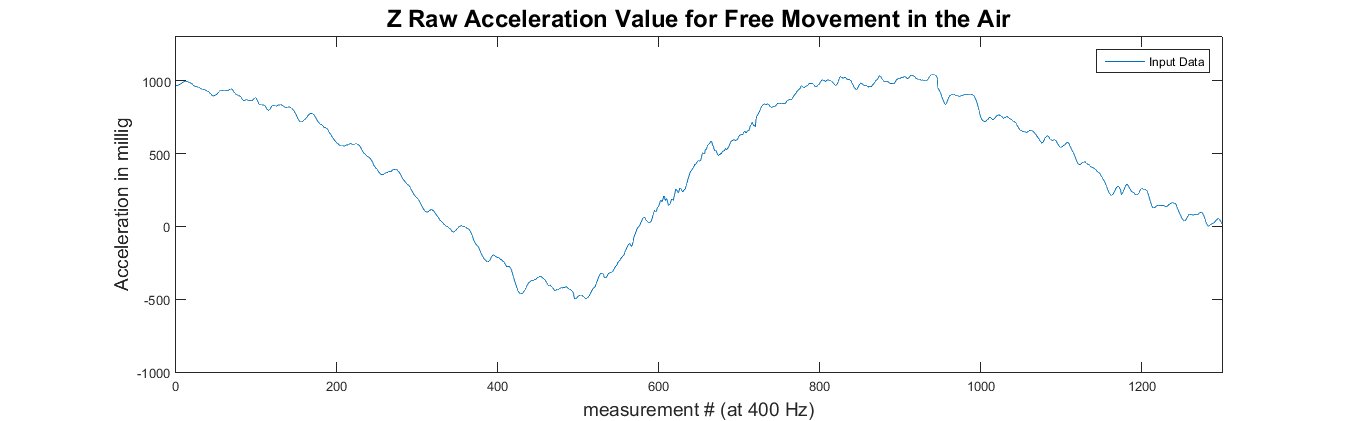
\includegraphics[scale=0.45]{images/DTcalibration3.png}
 \caption{Raw Acceleration Measurements from Free Movement in the Air}
 \label{fig:DTCAL3}
\end{figure}

\begin{itemize}
\item From figure \ref{fig:DTCAL1}, it was noted that a simple detection of a significant positive variation immediately followed by a significant negative variation could be used to detect a spike. The polling frequency of the accelerometer had to be increased from 25 Hz to 400 Hz in order to capture all the spikes without fail.
\item From figure \ref{fig:DTCAL1} again, some ringing was noticed after a tap. To avoid detecting multiple spikes from one tap while maintaining a low threshold value for the amplitude of the spike, a delay where no spikes are detected was added.
\item From figure \ref{fig:DTCAL2}, it can be noticed that just sliding the board on the table generates multiple spikes. To make sure these vibrations would not trigger a DT, a condition was implemented where if too many spikes were detected in the interval of time of a tap, the DT would not be counted.
\item From figure \ref{fig:DTCAL3}, it can be seen that the variation when moving the board in the air is not as fast as a spike. Hence having a high frequency polling and a high enough amplitude can filter this out.

\end{itemize}
\paragraph{}
After multiple hours of testing and adjusting of the parameter such as the amplitude and the time delays, a great DT detection algorithm was achieved. False positive from vibrations and random movements for three minutes intervals occurred on average 1.75 times.

\section{Timeline and Work Breakdown Between Team Member}
Work was heavily divided to ensure the best use of our time for this project. Félix Dubé mostly designed the whole android application with its elegant UI and took care of the Bluetooth communication protocol. Auguste Lalande took care of the SPI communication between the boards. Juan Morency Trudel developed the filtering algorithm for double tap detection and implemented the different LED modes with PWM. This segregation of the task was very efficient and allowed the project to be completed with an average of 10 hours of work per member. An overview of the time flow of the project is given in figure \ref{fig:Gantt} where days 28-31 are for the month of March and the following dates are for the month of April.
\begin{figure}[!htb]
 \centering
 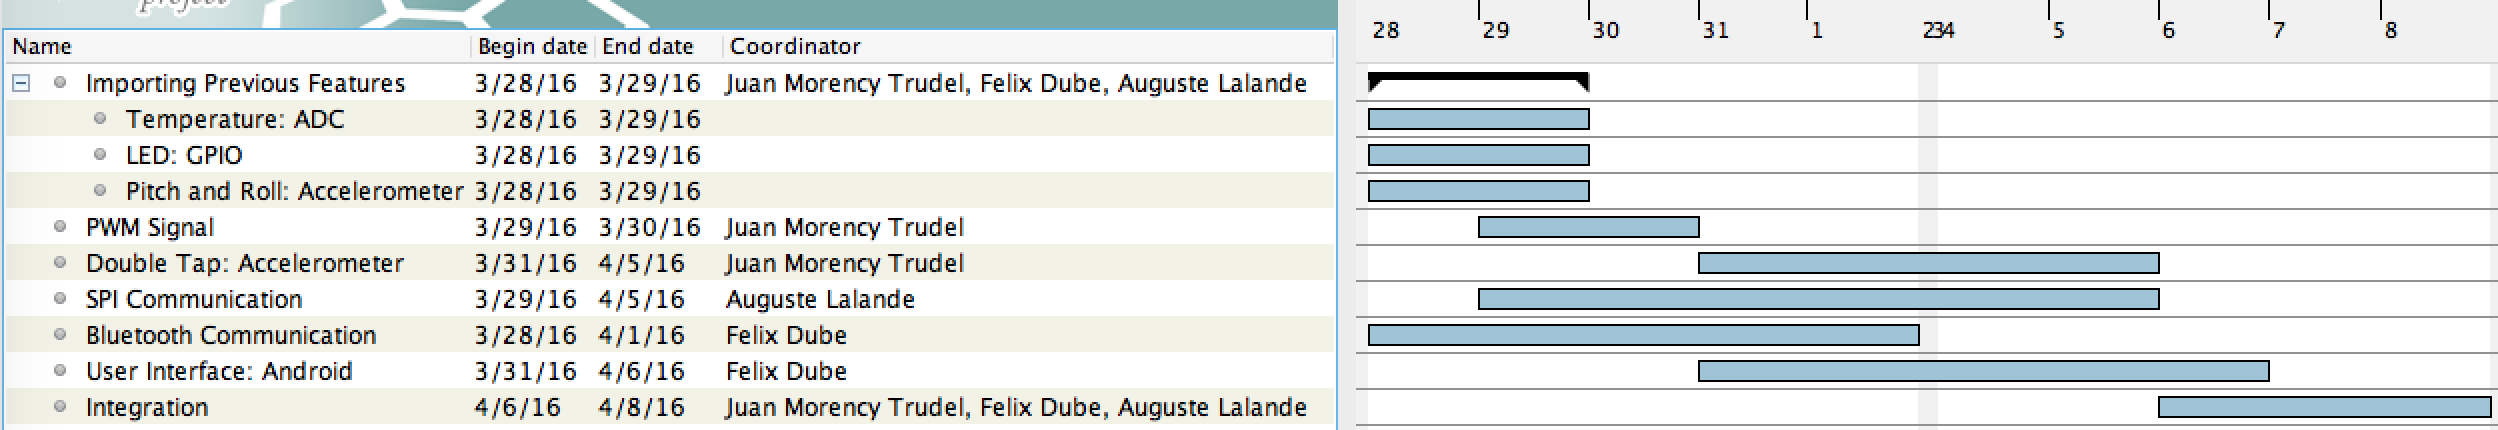
\includegraphics[scale=0.38]{images/gantt.png}
 \caption{Gantt Chart of the Project}
 \label{fig:Gantt}
\end{figure}
\section{Conclusion}
Wireless data acquisition and control of an embedded microcontroller with an android application was successfully implemented on a three device system. Results show that the robustness and flexibility of the BLE and SPI communication protocols justified their use. The appealing UI of the android application allowed easy monitoring of the temperature, pitch and roll angles of the discovery board with graphs as well as easy control of the brightness and rotation speed of the LED with sliders. Furthermore, the DT algorithm demonstrated a responsive and sensitive wake up feature of the phone. The control and monitoring of the embedded system with cellphone applications is rapidly becoming important in many fields in consumer electronics, such as routers, printers and Bluetooth speakers to name a few. The system presented in this report offers an easy and elegant approach to the communication required for such devices and should be considered for the many smartphone application projects to come.


\newpage
\section{Bibliography}
\bibliographystyle{unsrt}
\bibliography{ProjectReport}

\newpage
\section{Appendix}
\begin{figure}[!htb]
 \centering
 \includegraphics[scale=0.6]{images/softwareArchitecture.png}
 \caption{High Level View of the Software Architecture}
 \label{fig:softArch}
\end{figure}


\begin{figure}[!htb]
 \centering
 \includegraphics[scale=0.50]{images/FSMDT.png}
 \caption{Finite State Machine of the Filtering Algorithm Required for Double Tap Detection}
 \label{fig:FSMDT}
\end{figure}


\end{document}
